\chapter {Introduction and motivation}

In classical physics a neutral particle can have an \gls{edm} caused by separation of charge, with dimensions of charge-length. The classical equation that defines an \gls{edm}, $\vec{d}$, is given by
\begin{equation}\label{eq:pEDM}
    \vec{d} = \int_V \rho (\vec{x})\vec{x} d^3\vec{x},
\end{equation}
% Additionally, a charged particle can have an \gls{edm}, which is related to a separation between its center of charge and center of mass % not as clear as I would've hoped
where the EDM of the particle or any system of particles is given by $\vec{d}$, and is non-zero only when there is a non-symmetric electric charge density, $\rho(\vec{x})$ over its volume, $V$.

The intrinsic EDM differs from Eq. \ref{eq:pEDM}. At low energies, the Hamiltonian of a particle with spin $\vec{J}$, a magnetic moment $\vec{\mu}$, and an intrinsic \gls{edm} $\vec{d}$, in the presence of an electric field $\vec{E}$, and magnetic field $\vec{B}$, can be described by
\begin{equation} \label{eq:hamiltonian}
    \hat{H} = -\vec{d} \cdot \vec{E} - \vec{\mu} \cdot \vec{B}=-d \frac{\vec{J}}{J}\cdot \vec{E} - \mu \frac{\vec{J}}{J}\cdot \vec{B}.
\end{equation}
It is important to note that the spin vector $\vec{J}$ is parallel both the EDM $\vec{d}$, and magnetic moment, $\vec{\mu}$. 

Searches for \gls{edm}s intrinsic to particles have been made since the 1950s and continue today, as shown in Fig. \ref{fig:EDMsearch}. These searches are described in the reviews by Chupp et al. \cite{Chupp2019}, Pospelov and Ritz \cite{Pospelov2005}, and Engel, Ramsey-Musolf, and van Kolck \cite{Engel2013}. The search for an intrinsic EDM was initiated by looking at the neutron as a possible source of parity-violation (P-violation). Parity symmetry (P-symmetry) is invariant under mirror reflection, and was once thought of as a fundamental symmetry of nature. P-symmetry was first found to be violated maximally in measurements of the Cobalt-Nickel $\beta$-decay and was later found to be violated maximally for weak force interactions. Under the parity operator $\mathcal{P}$, polar vectors change direction, but not axial vectors. The vectors $\vec{d}$, $\vec{\mu}$ and $\vec{B}$ remain unchanged under $\mathcal{P}$ since they are axial vectors, but the polar vector $\vec{E}$ reverses sign. An \gls{edm} is a P-odd as shown in Eq. \ref{eq:PVedm}.

A \gls{edm} is not only P-violating but also a time-violating (T-violating). This is because under the time reversal operator $\mathcal T$, the axial vectors $\vec{\mu}$, $\vec{B}$, and $\vec{d}$ must change sign, while the electric field $\vec{E}$ remains unchanged. Under the $\mathcal{T}$ operator the equation of motion follow a different Hamiltonian, hence T-symmetry is violated, as illustrated by

\begin{equation} \label{eq:PVedm}
\begin{split}
     \hat{H} \neq \mathcal{P}(\hat{H}) = -\vec{d} \cdot (-\vec{E}) - \vec{\mu} \cdot \vec{B} \; \textrm{and} \\
    \hat{H} \neq \mathcal{T}(\hat{H})= -(-\vec{d}) \cdot \vec{E} - (-\vec{\mu}) \cdot (-\vec{B}). 
\end{split}
\end{equation}

There is one more operator to discuss, the conjugate charge $\mathcal{C}$ operator and its related symmetry. A physics variable with Charge conjugate symmetry is invariant to a change from particle to the respective antiparticle. Each of the individual symmetries T, P, and C were once thought of as good symmetries, and physics was thought to be invariant under each of the related operators. But each symmetry was found to be violated. The weak force violates P-symmetry and C-symmetry maximally. The combined CP symmetry was though of as a good symmetry but then K-$\bar{\textrm K}$ oscillation was discovered. Each time a new symmetry violation was observed, the \gls{sm} had to modified to explain the finding. The combined CPT symmetry is now thought to be a good symmetry of the universe. CPT symmetry relies on Lorentz invariance in relativistic quantum theories to hold true, and is necessary to explain currently accepted relativistic quantum theories. Under CPT theorem a T-violating process is also a a CP-violating process. 

Motivation for the \gls{edm} search is to discover new sources of C-violation and CP-violation. The CPT theorem suggests that an atomic EDM that violates T-symmetry is also a CP-violating process. Sources of direct C-violation and CP-violation in the universe help explain baryogenesis. Baryogenesis is the preferred creation of baryons over antibaryons. This baryon preference left the remnant matter in the universe that is observed today. Andrei Sakharov proposed a set of three conditions in 1967 which the processes that generate baryons must follow in order to produce the matter-antimatter asymmetry currently observed in the universe \cite{Sakharov}. The conditions state that there must be

\begin{enumerate}
    \item a Baryon non-conserving process,
    \item C and CP-violating processes, and 
    \item interactions out of thermal equilibrium.
\end{enumerate}

The first Sakharov condition is the most obvious. In order for there to be a baryon asymmetry from an originally symmetric universe there must also be a process that does not conserve the baryon number. If the baryon number conservation was not violated then parts of a symmetric universe would have annihilated moments after the Big Bang. Such annihilation would leave detectable signals currently absent from cosmic observations. The alternative to baryogenesis is that the universe was created with some amount of baryonic matter, however this remains an unattractive theory. Currently, baryogenesis is more favorable theoretically. The observed baryon asymmetry today is
\begin{equation}
    \frac{n_B- n_{\overline{B}}}{n_\gamma} \approx 10^{-10},
\end{equation}
which is larger by orders of magnitude than the asymmetry predicted by the \gls{sm}s electroweak baryogenesis. Here $n_B$ is the baryon density, $n_{\overline{B}}$ is the antibaryon density and $n_\gamma$ is the photon density.  Electroweak baryogenesis is the \gls{sm}'s version of baryogenesis. It is because the Sakharov conditions of baryogenesis and the apparent lack of CP-violation in the \gls{sm} that searches for CP-violation are a good physics motivation.

The standard model can account for the EDM only via a CP-violating phase in the Cabibbo-Koybayashi-Maskawa (CKM) matrix, and the $\bar{\theta}_{\textrm{QCD}}$ term. However, the CKM phase contributions to \gls{edm}s are small compared to current and ongoing \gls{edm} search sensitivities. The \gls{qcd} contributions are highly constrained by \gls{edm} measurements. The apparent lack of CP-violation in the strong force is known as the strong CP problem. This is a problem because the dimensionless parameters $\theta$ can be any number and on the grounds of naturalness would be assumed to be of order 1.  However, neutron EDM measurements constrain $\theta$ to be less that $10^{-10}$.

\begin{figure} [htbp]
	\center
	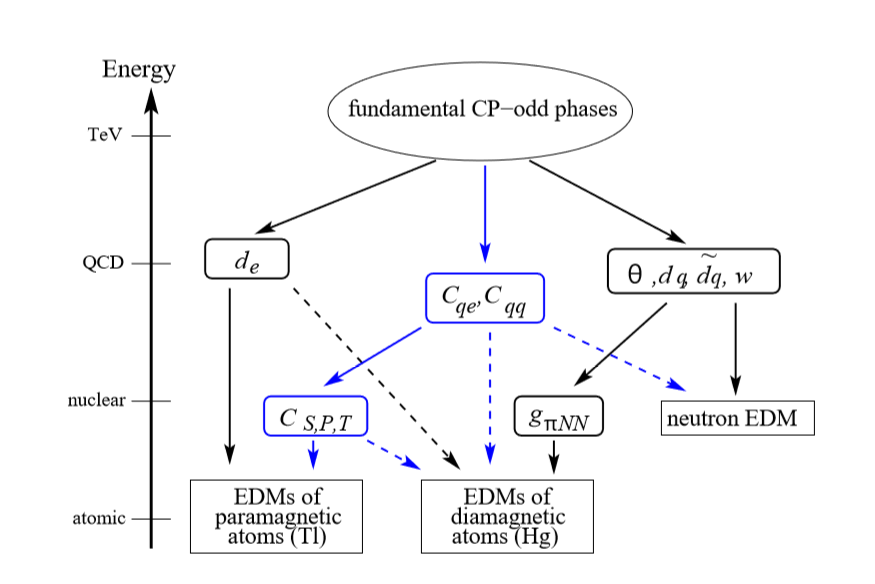
\includegraphics[width=0.8
	\textwidth]{OverviewPicture.png}
	\caption { A schematic plot of the scales between CP-odd sources from the physics review by Pospelov and Ritz \cite{Pospelov2005} shows how new physics from the TeV scale interactions feeds into operators and parameters at the scales of \gls{qcd}, nuclear physics and atomic energy scales, the solid lines represent the important contributions that lead directly from one level to another.}
		\label{fig:EDMsource}
\end{figure}

Fundamental theories set the scale of an EDM, or are have parameters that set the strength of CP-odd process that give rise to the EDM. Fig. \ref{fig:EDMsource} shows the contributions to atomic \gls{edm} from the atomic, nucleon, and QCD energy levels being fed by fundamental CP-odd phases. At the atomic level the atom can be either paramagnetic (spin-1/2 electron unpaired) or diamagnetic (spin-0 pair of electrons). 

The paramagnetic atoms directly couple to the electron  \gls{edm} $d_e$, with connections from nuclear effects $C_{S,P,T}$. Here $C_{S,P,T}$ are quark-electron coupling strength $C_{qe}$ for \gls{qcd} expressed as an effective field theorem at the nuclear scale. For diamagnetic atoms the picture is more complicated, and in addition to contributions to their \gls{edm} that are the same as in the paramagnetic case, they have contributions from $g_{\pi NN}$ coupling constant between pions and the nucleons in the nucleus, the quark EDM $d_q$, and the strong-CP phase $\theta$. 

The CP-odd parameters and interaction give rise to the EDMs of these observables at the atomic level. Specifically, looking at the effective field theory Lagrangian at the nuclear scale level: there are the direct contributions from particles such as the neutrons, proton and the electron EDMs; the CP-violating electron-nucleon and nucleon-nucleon interactions; and the CP-odd pion-nucleon interactions. The second term can be though of as the nucleon induced EDM. The Lagrangian is given by

\begin{equation}
    \begin{split}
        \mathcal{L}^{\textrm{nuclear}}_{eff} =  \mathcal{L}_{\textrm{edm}} (d_e, \, d_n, & \, d_p)+  \mathcal{L}_{\pi \textrm{NN}}(\bar{g}^{(0)}_{\pi \textrm{NN}}, \, \bar{g}^{(1)}_{\pi \textrm{NN}}, \, \bar{g}^{(2)}_{\pi \textrm{NN}} )\\+ 
        & \mathcal{L}_{eN}(C_{\textrm{S}}, \, C_{\textrm{P}}, \, C_{\textrm{T}}).
    \end{split}
\end{equation}
%with the specific therms given by:
%\begin{equation}\label{eq:Ledm}
%    \mathcal{L}_{\textrm{edm}}=-\frac{i}{2} \sum_{i=e,p,n}d_i\bar{\psi_i}(F\sigma)\gamma_5 \psi,
%\end{equation}
%
%\begin{equation}\label{eq:Lpnn}
%    \mathcal{L}_{\pi \textrm{NN}}=
%    \bar{g}^{(0)}_{\pi \textrm{NN}} \bar{\textrm{N}} \tau^a \textrm{N}\pi^a+\bar{g}^{(1)}_{\pi \textrm{NN}} \bar{\textrm{N}}\textrm{N}\pi^0
%    +
%    \bar{g}^{(2)}_{\pi \textrm{NN}}( \bar{\textrm{N}} \tau^a \textrm{N} \pi^a-\bar{\textrm{N}}\tau^3\textrm{N}\pi^0),
%\end{equation}%
%
%\begin{equation}\label{eq:Len}
%    \begin{aligned}
%           \mathcal{L}_{e\textrm{N}}={}&
%    C^{(0)}_{\textrm{S}} \bar{e}i\gamma_5 e  \bar{\textrm{N}}\textrm{N}+ C^{(0)}_{\textrm{P}} \bar{e} e  \bar{\textrm{N}} i\gamma_5\textrm{N}
%    +   C^{(0)}_{\textrm{T}}\epsilon_{\mu \nu \alpha \beta} \bar{e} \sigma^{\mu \nu} e  \bar{\textrm{N}} \sigma^{\alpha \beta}\textrm{N} \\
%    &+ C^{(1)}_{\textrm{S}} \bar{e}i\gamma_5 e  \bar{\textrm{N}}\tau^3 \textrm{N}
%    + C^{(1)}_{\textrm{P}} \bar{e} e  \bar{\textrm{N}} i\gamma_5\tau^3 \textrm{N}
%    + C^{(1)}_{\textrm{T}}\epsilon_{\mu \nu \alpha \beta} \bar{e} \sigma^{\mu \nu} e  \bar{\textrm{N}} \sigma^{\alpha \beta}\tau^3 \textrm{N}.
%    \end{aligned}
%\end{equation}
Succinctly, the Lagrangian $\mathcal{L}$ can be expressed as a set of interaction coefficients $\alpha_i$ of the interactions defined by CP-odd interaction operators $\mathcal{O}^{CP}_i$, where the subscript $i$ sums over all of the CP-odd interactions. The succinct form of the Langrangian is 
\begin{equation}
    \mathcal{L} = \sum_i \alpha_i \mathcal{O}^{CP}_i.
\end{equation}
 At the nuclear scale, the coefficients of the Lagrangian $\alpha$ have a complicated dependence on the observable atomic EDM. The dependence of the strength of interaction is a many body nuclear problem. 
 
 It is important to note that in addition to the electron EDM, $d_e$, the quark-quark and quark electron interactions $C_{qq}$, and $C_{eq}$ play an important role in determining the interactions that generate the EDM of paramagnetic atoms. The atoms of $^{129}$Xe or $^{199}$Hg are diamagnetic, but it is still important to discuss the physics for a paramagnetic atom. 
 
 The paramagnetic atom acquires an EDM from an unpaired relativistic electron that in the valance shell. The EDM grows stronger with increasing atomic number since the orbitals have higher atomic radius. The strength of EDM of paramagnetic atom is given by
\begin{equation}
    d_{para}(d_e) \sim 10 \frac{Z^3 \alpha^2}{J(J+1/2)(J+1)^2} d_e,
\end{equation}
where $Z$ is the atomic number, $J$ is the angular momentum quantum number, and $\alpha$ is the fine structure constant.

For diamagnetic atoms, the contributions to the  EDM are from a collection of relevant parameters, including the Schiff moment contribution from the nucleus
\begin{equation}
    d_{dia}=d_{dia}(S[\bar{g}_{\pi N N },d_N],C_S,C_p,C_T,d_e).
\end{equation}
Schiff's theorem states that a point-like nucleus in a non-relativistic cloud of electrons would experience negligible nuclear EDM due to the screening of the nuclear EDM from the electrons. A Schiff moment is the name given to the EDM moment that violates Schiff's Theorem. In the nucleus P-odd and T-odd nucleon-nucleon interactions $g_{\pi N N}$ lead to CP-violation. Finite sized nuclei violate Schiff's theorem because the electrons can be relativistic, and the nucleus may not be symmetric \cite{Flambaum, Sushkov}.

Typical beyond standard model theories predict a larger EDM than predicted in the SM. So far only limits on EDM have been placed, leading to upper bounds on particle \gls{edm}s, which can be interpreted as limits on the parameters of the beyond standard model physics.
%Why focus on Diamagnetic and neutron EDM